The RTSC board contains a 54-pin, ball grid array (BGA) packaged MT45W8MW16BGX 128Mbit DRAM IC from Micron\textsuperscript{\textregistered} with its address and data bus connected in parallel with a JS28F128 128Mb Flash ROM fron Intel\textsuperscript{\textregistered}~\cite{DigilentNexys2rm}.  The DRAM is used by the configuration on the FPGA to store stimulation waveform data, and the Flash ROM is not used~\cite{BatzerMSEE}.  Figure~\ref{fig:dram} shows the connections between the Xilinx\textsuperscript{\textregistered} XC3S500E FPGA and the DRAM and Flash ROM on the RTSC board.

\begin{figure}[htb]
	\begin{singlespace}
	\centering	
		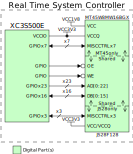
\includegraphics{./figures/DRAM} 
	\caption{Connections between the FPGA and the DRAM and Flash memory ICs on the RTSC board~\cite{DigilentNexys2rm,DigilentNexys2sch}\label{fig:dram}}
	\end{singlespace}
\end{figure}

The DRAM requires a $+1.8\unit{V}$ power supply for its internal circuitry and has a dedicated supply pin for interface logic as described in section~\ref{sec:rtscpower}.  Seven control signals are connected exclusively between the FPGA and DRAM IC.  The 23-bit wide address bus, 16-bit bi-directional data bus, output enable ($\overline{\mathrm{OE}}$) signal, and write enable ($\overline{\mathrm{WE}}$) signal are connected to both the DRAM and Flash IC.  The Flash IC has a 25-bit address bus, but its MSbit and LSbit are pulled LOW~\cite{DigilentNexys2sch}.  Three control signals are connected exclusively between the FPGA and Flash ROM IC.